\subsection{Probleme bei der Zahlenerkennung}\label{sec:problem_number_detection}
Bei der Verarbeitung der Bildausschnitte wird der jeweilige Ausschnitt verkleinert, um mit den Trainingsdaten übereinzustimmen. Dieser Schritt ist notwendig, da der SVM Algorithmus mit Bildern trainiert wurden, die alle eine Größe von 8×8 Pixeln haben. Die Größe der Bilder gibt dabei auch die Anzahl der Gewichte wieder, bei 8×8 großen Bildern sind es 64 Gewichte, bei 12×12 Pixeln wären es demnach 144 Gewichte und bei 28×28 Pixeln 784 Gewichte. Pro Pixel wird also jeweils ein Gewicht trainiert.\par
Bei dem Erkennen eines Bildes wird nun jeder Pixel überprüft, welche Farbe, in diesem Falle schwarz oder weiß, er besitzt. Je nach Anordnung erkennt jetzt der Algorithmus eine oder mehrere Zahlen. Da nicht jede Zahl immer gleich geschrieben ist, gibt es Pixel, die in jedem Fall eine Farbe haben müssen und andere wiederum können schwarz sein oder eben nicht. Diesen Wert geben die Gewichte des jeweiligen Pixels an. Bei einer 8 ist z.B. der Punkt in der Mitte immer schwarz. Der Bereich im oberen und unteren Kringel wiederum hat keine festgelegte Farbe, da es an dieser Stelle bei vielen verschiedenen Handschriften für diese Zahl kein einheitliches Muster gibt, sondern mal mehr und weniger weiße Fläche. Bei einer 1 hingegen wäre der Bereich unten links immer weiß. \par
Da es nun bei unterschiedlichen Zahlen auf einzelne Gewichte und wie diese trainiert sind ankommt, kann es schnell passieren, dass es bei ähnlichen Zahlen zu Verwechslungen kommt. Vergleicht man z.B. eine 8, siehe \ref{fig:8_in_8x8_grid}, und eine 3, siehe \ref{fig:3_in_8x8_grid}, fällt  auf, dass sie sich nur um 2 Pixel unterscheiden. Hierbei kommt es natürlich immer darauf an, wie die Zahl geschrieben wurde.\par
\begin{figure}[H]
    \begin{subfigure}{.5\textwidth}
        \centering
        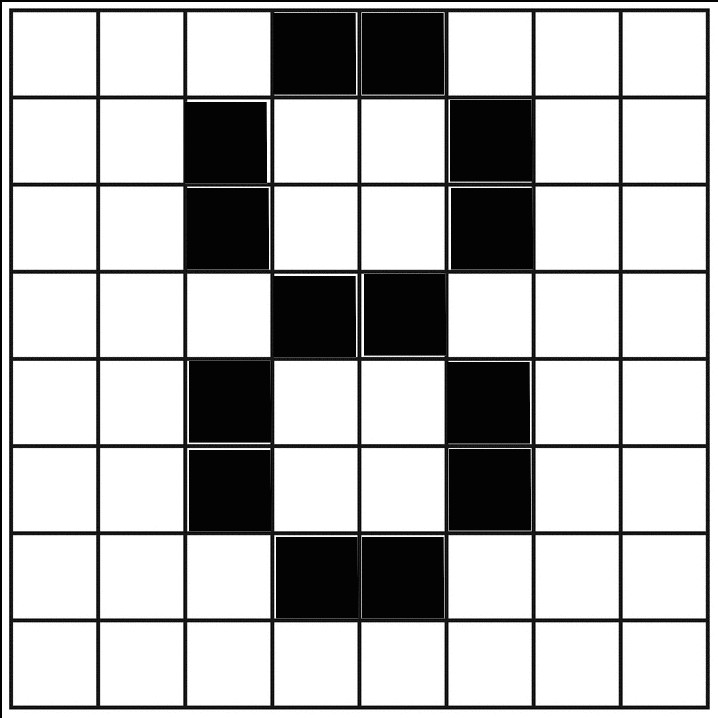
\includegraphics[width=.8\linewidth]{images/practice/numbers/8_in_8x8_grid.jpg}
        \caption{8 in einem 8×8 Gitter}
        \label{fig:8_in_8x8_grid}
    \end{subfigure}%
    \begin{subfigure}{.5\textwidth}
        \centering
        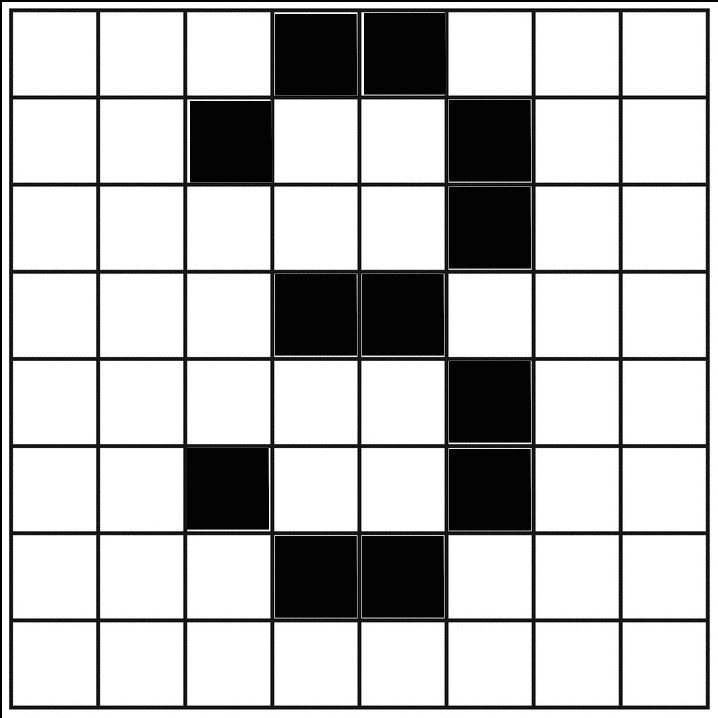
\includegraphics[width=.8\linewidth]{images/practice/numbers/3_in_8x8_grid.jpg}
        \caption{3 in einem 8×8 Gitter}
        \label{fig:3_in_8x8_grid}
    \end{subfigure}
    \caption{Zaheln in einem 8×8 Gitter}
    \label{fig:8x8_grid}
\end{figure}
Je nachdem wie nun die Trainingsdaten des Algorithmus aussahen kann es sein das die Gewichte trainiert wurden, um beides als dieselbe Zahl zu erkennen. Da es in diesem Beispiel nur von einem einzigen Gewicht abhängig ist, ist das sogar wahrscheinlich.\par
Nutzt man jedoch stattdessen Bilder mit einer besseren Auflösung, also mit mehr Pixeln, kann das nicht so einfach passieren. Wie in \ref{fig:28x28_grid} zu sehen unterscheiden sich die beiden Bilder um 18 Pixel, statt wie zuvor nur um 2 Pixel. Diese 18 Pixel bilden nun nicht nur einen größeren weißen Bereich, sondern es braucht auch mehr als nur ein einzelnes Gewicht, um die Vorhersage zu ändern. Außerdem ist auch, aufgrund der höheren Gesamtanzahl von Gewichten, der Einfluss eines einzelnen Gewichts auf das Gesamtergebnis geringer.\par
\begin{figure}[H]
    \begin{subfigure}{.5\textwidth}
        \centering
        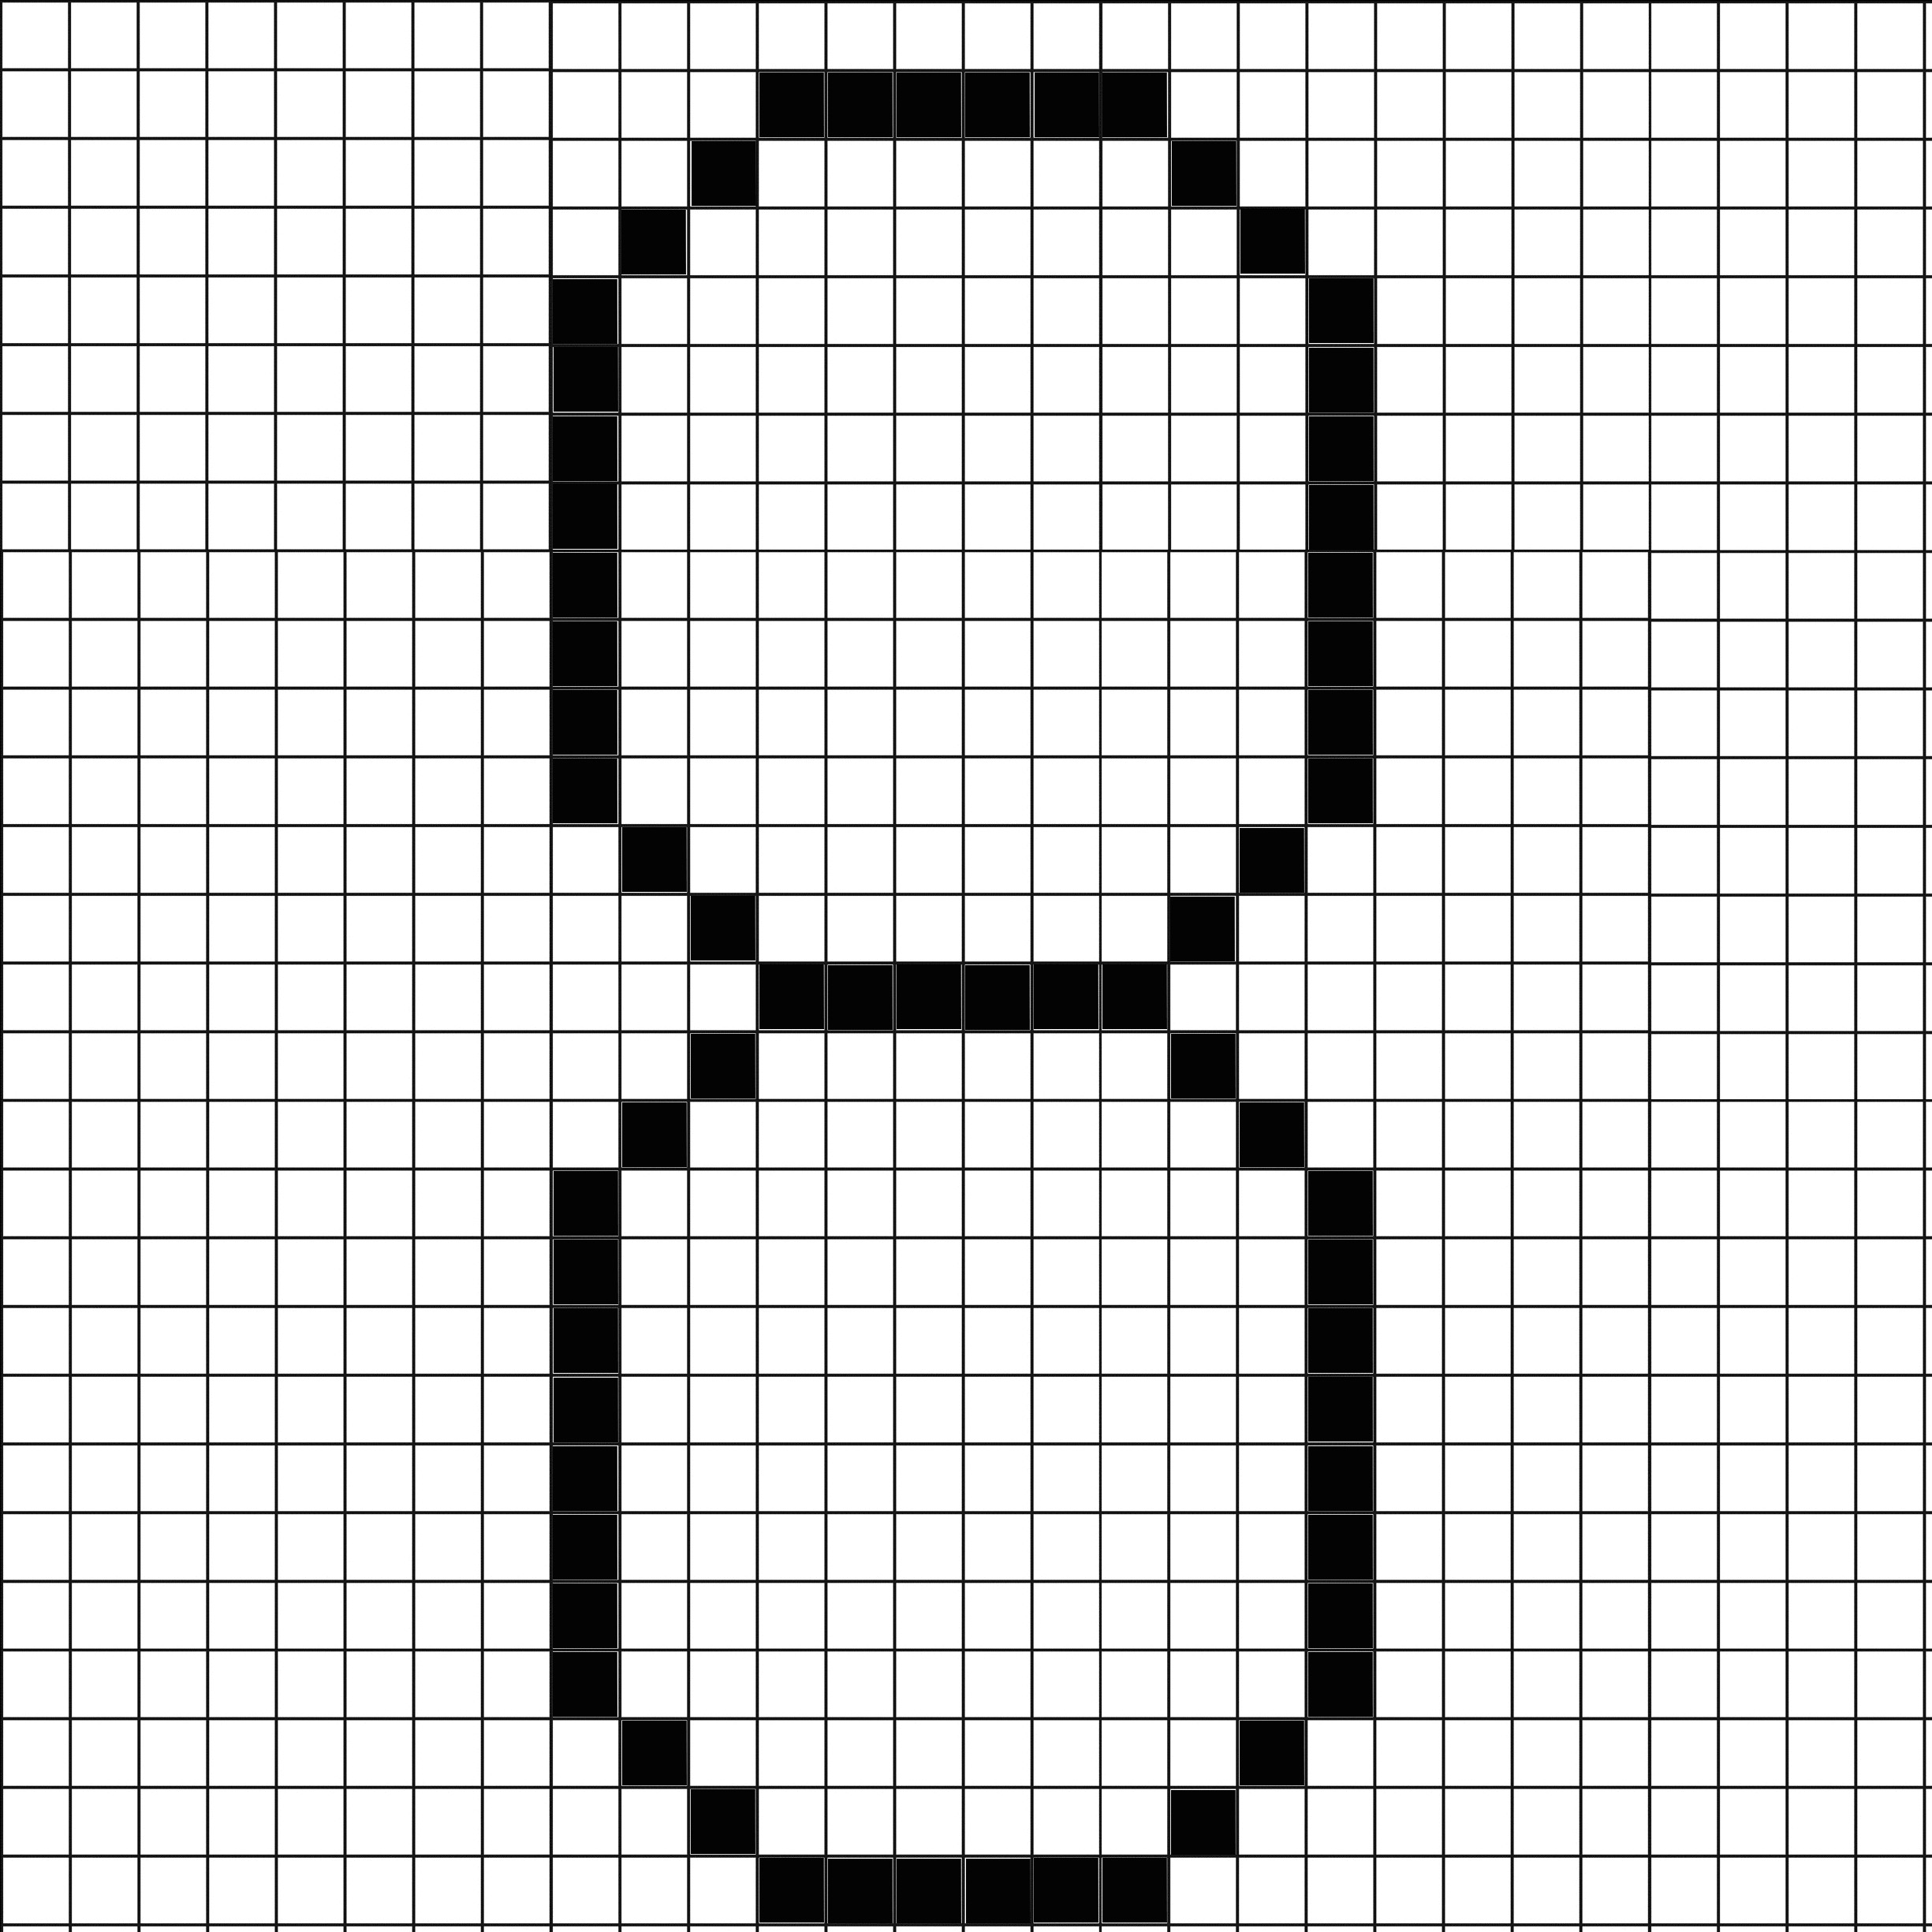
\includegraphics[width=.8\linewidth]{images/practice/numbers/8_in_28x28_grid.jpg}
        \caption{8 in einem 28×28 Gitter}
        \label{fig:8_in_28x28_grid}
    \end{subfigure}%
    \begin{subfigure}{.5\textwidth}
        \centering
        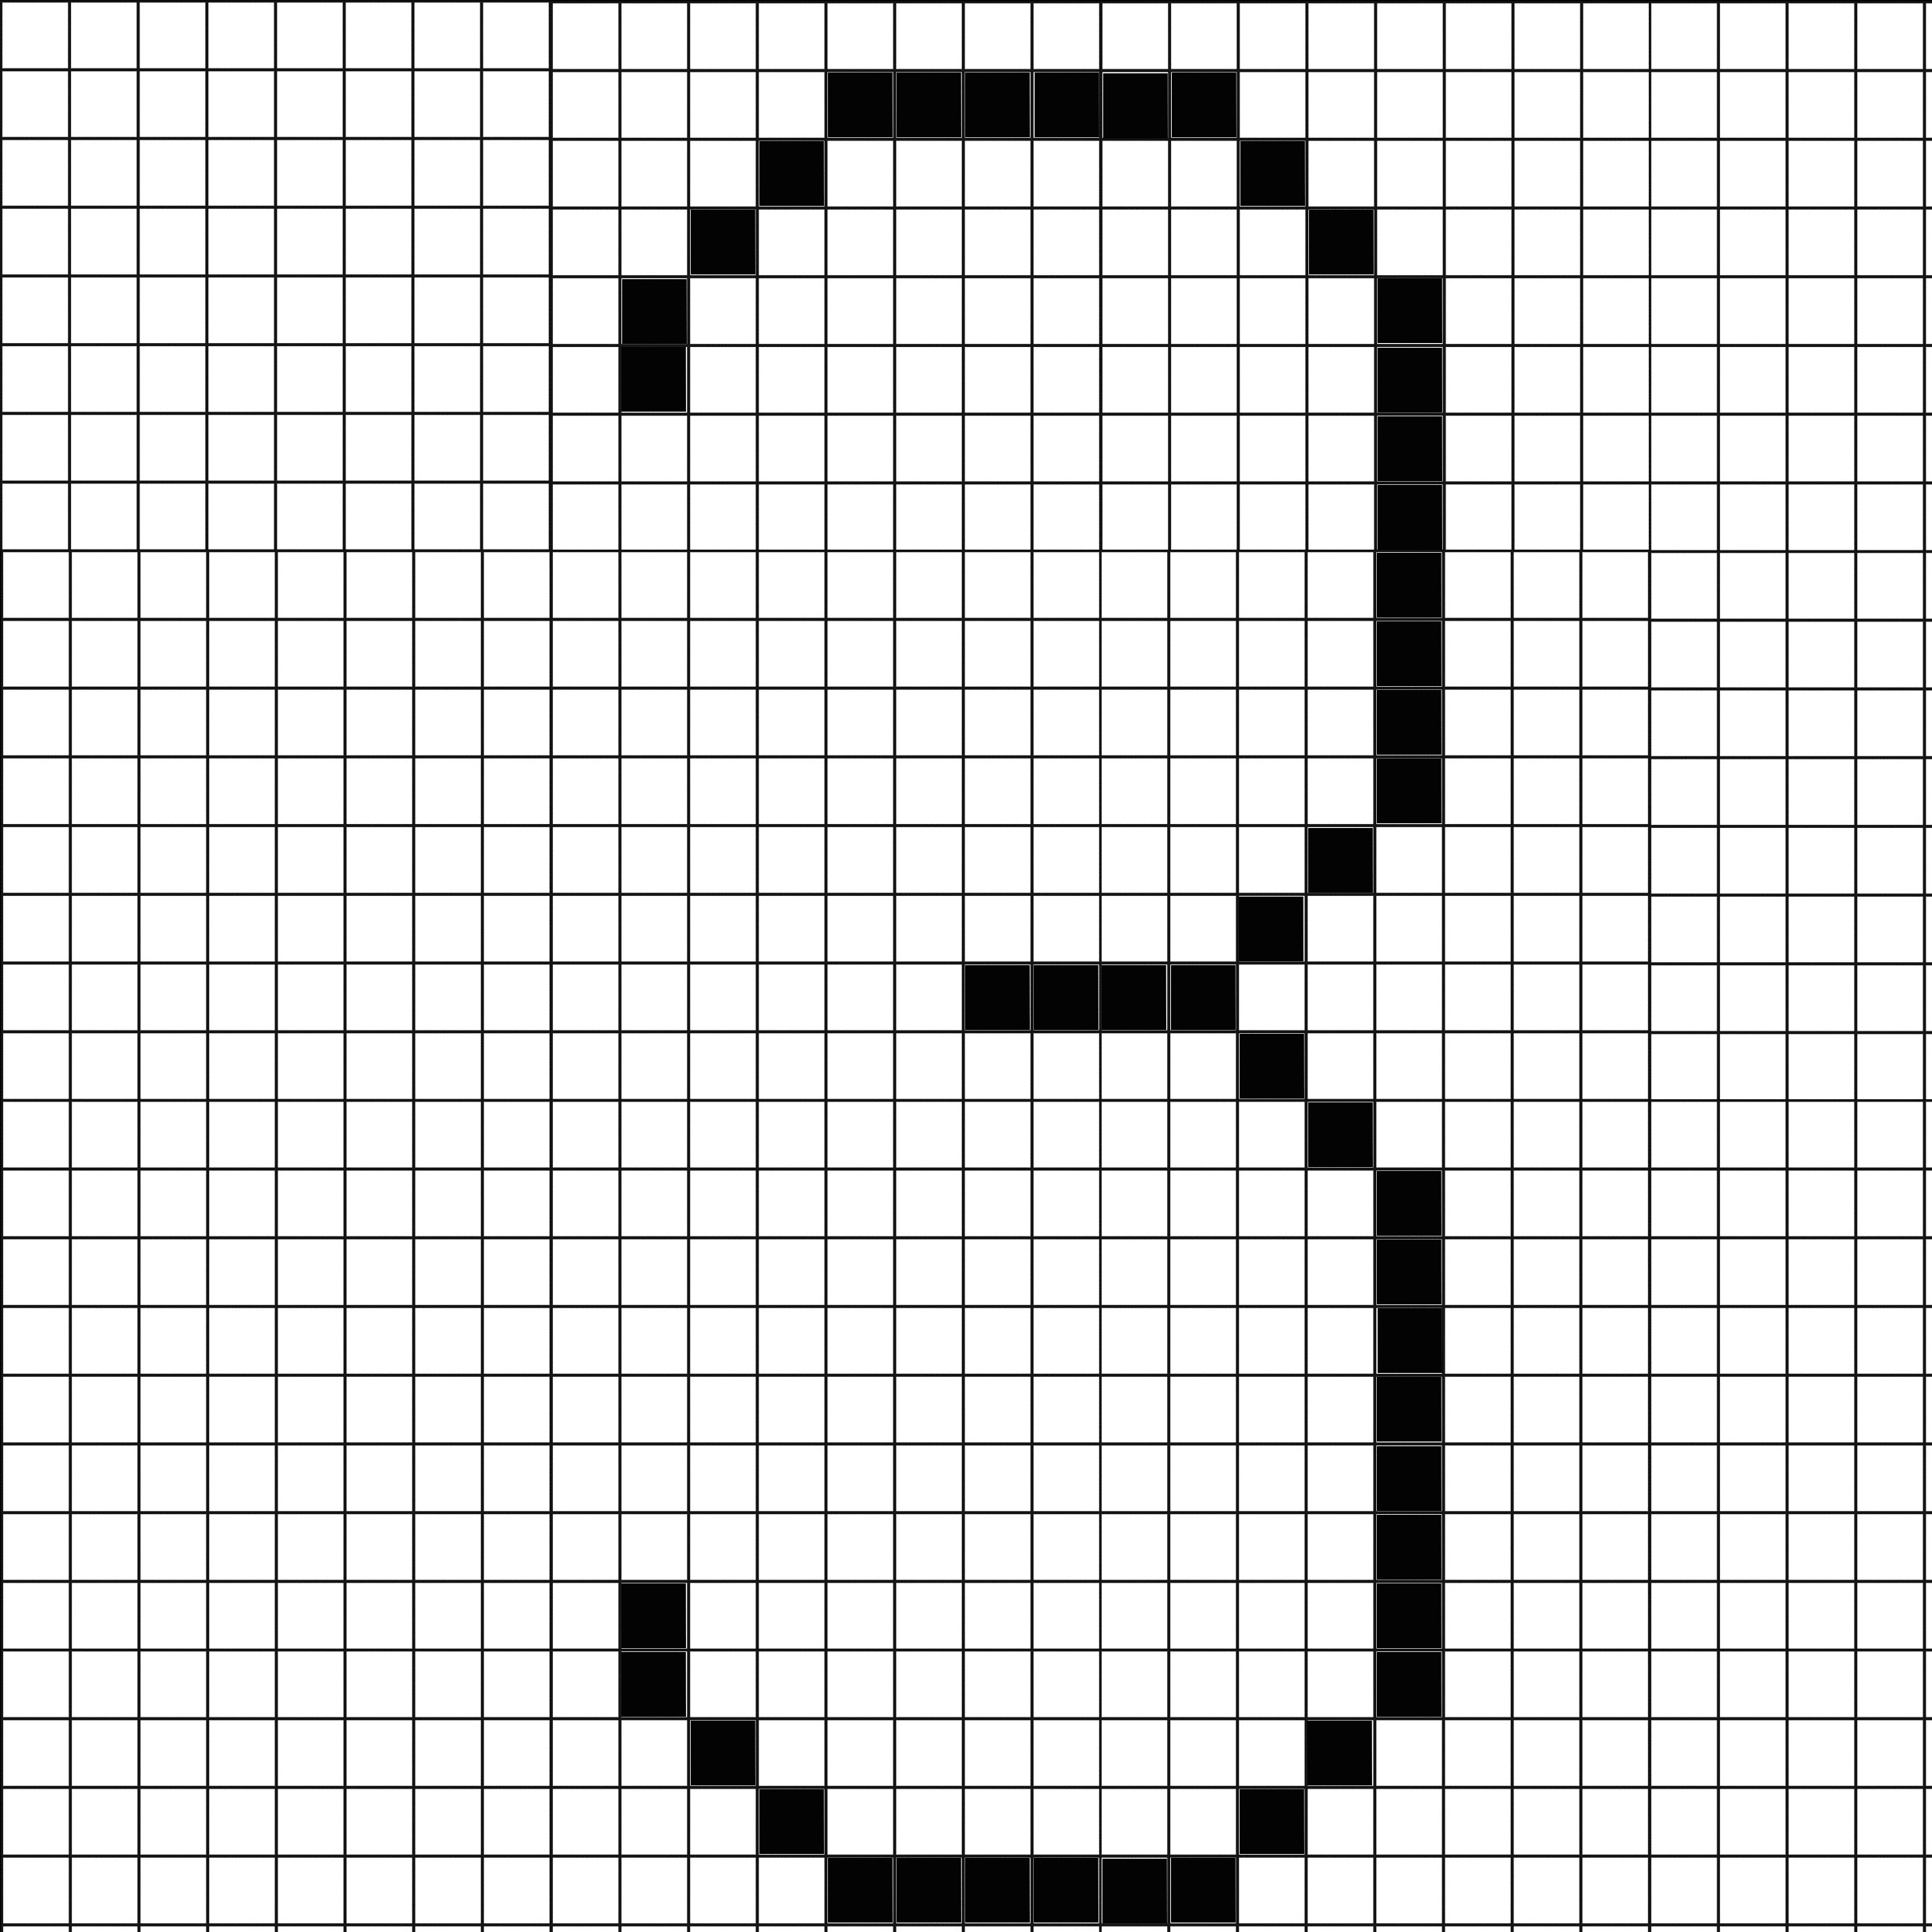
\includegraphics[width=.8\linewidth]{images/practice/numbers/3_in_28x28_grid.jpg}
        \caption{3 in einem 28×28 Gitter}
        \label{fig:3_in_28x28_grid}
    \end{subfigure}
    \caption{Zaheln in einem 28×28 Gitter}
    \label{fig:28x28_grid}
\end{figure}

Dabei ist natürlich zu beachten, dass es für wirklich handgeschriebene Zahlen noch mehr Einflussfaktoren wie die bloße Farbe der Pixel gibt und auch jeder Mensch die Zahlen anders schreibt.\par

Allerdings haben diese zusätzlichen Gewichte auch einen großen Nachteil, da sie die Komplexität des Algorithmus erhöhen. Der SVM-Algorithmus ist bei den kleinen 8×8 Bilder, selbst bei weniger leistungsstarken Geräten, innerhalb von Millisekunden bis wenige Sekunden trainiert und einsatzbereit. Es wäre also möglich jederzeit neu zu trainieren ohne das es großen Einfluss auf die Nutzung der Anwendung hat. Wie in \ref{ssec:eval} zu sehen ist, besitzt er eine sehr gute Genauigkeit, weshalb sich auch zu Recht für diesen Algorithmus entschieden wurde. \hfill \\
Einen SVM-Algorithmus der hingegen mit Bildern der Größe 28×28 trainiert wird benötigt ungefähr 7 Minuten, es wäre also nicht möglich den Algorithmus mal schnell neu zu trainieren.\par

Aber, wie bereits erwähnt, muss jedes Bild, das dem Algorithmus zur Klassifizierung übergeben wird, zuvor auf die Größe von 8×8 Pixeln reduziert werden. Um dies zu erreichen, wird eine sogenannte Interpolation durchgeführt. Dabei wird aus den Farbwerten mehreren benachbarten Pixeln ein neuer Wert berechnet und somit vereint. Durch diesen Schritt kommt es allerdings zu Informationsverlust. Je größer der Unterschied zwischen dem Originalbild und dem Resultat ist, desto mehr Informationen gehen dabei verloren. Dies kann so weit gehen, dass am Ende nicht mal mehr eine Zahl zu erkennen ist und das Ergebnis der Klassifizierung nur geraten ist.\par

Trainiert man nun den SVM-Algorithmus mit einem Datensatz von 28×28 großen Bilder besitzt er, selbst mit mischen der Test- und Trainingsdaten, nur noch eine Genauigkeit von 94\%.\par
\begin{minipage}{\textwidth}[H]
    \begin{lstlisting}[language=Bash, caption=Testergebnisse der SVM mit 28x28 großen Bildern, label=lst:testergebnis_svm_groß]
Klassifizierungsbericht SVC(gamma=0.001):
              precision    recall  f1-score   support

         0.0       0.96      0.99      0.97       980
         1.0       0.97      0.99      0.98      1135
         2.0       0.94      0.92      0.93      1032
         3.0       0.93      0.94      0.93      1010
         4.0       0.92      0.95      0.94       982
         5.0       0.92      0.91      0.92       892
         6.0       0.95      0.96      0.96       958
         7.0       0.95      0.93      0.94      1028
         8.0       0.93      0.91      0.92       974
         9.0       0.94      0.91      0.92      1009

    accuracy                           0.94     10000
   macro avg       0.94      0.94      0.94     10000
weighted avg       0.94      0.94      0.94     10000

Genauigkeit:  0.9415
	\end{lstlisting}
\end{minipage}
Allerdings beinhaltet, wie sich an dieser Stelle herausgestellt hat, der in \textit{Keras} vorhandene Datensatz bereits ausschließlich Bilder der Größe 28×28. Besagter Datensatz wurde verwendet, um den \textit{CNN} zu trainieren und dieser hat mit 99,16\%, siehe \ref{lst:test_cnn_results}, eine höhere Genauigkeit als der SVM-Algorithmus. Die um 5\% höhere Genauigkeit kann bei der Benutzung der Anwendung einen entscheidenden Einfluss haben, wohingegen die Einfachheit der Umsetzung nur beim ersten Entwickeln des Algorithmus von Bedeutung ist. Aus diesem Grund ist es sinnvoll für die Klassifizierung der Zahlen den \textit{CNN} anstatt des \textit{SVM-Algorithmus} zu verwenden.
